\documentclass[11pt,a4paper]{article}

\usepackage[T1]{fontenc}
\usepackage[utf8]{inputenc}
\usepackage{lmodern}
\usepackage[margin=2.5cm]{geometry}
\usepackage{amsmath,amssymb}
\usepackage{graphicx}
\usepackage{booktabs}
\usepackage{array}
\usepackage[font=small,labelfont=bf]{caption}
\usepackage[numbers,sort&compress]{natbib}
\usepackage{microtype}
\usepackage[hidelinks]{hyperref}
\usepackage{xurl}

\graphicspath{{figures/}}

% Numbers quoted in the text, generated from data/*.npz by paper/make_figures.py
% Generated by paper/make_figures.py from data/*.npz. Do not edit.
\newcommand{\aTheory}{48.25}
\newcommand{\basesErrMax}{0.36}
\newcommand{\basesErrMin}{0.15}
\newcommand{\basesHidden}{96}
\newcommand{\basesResMax}{9,979}
\newcommand{\basesResMin}{2,536}
\newcommand{\dAICcExt}{1.8}
\newcommand{\dLIngard}{1.43}
\newcommand{\dLIngardInt}{0.58}
\newcommand{\dLext}{1.56}
\newcommand{\dLextGap}{3}
\newcommand{\dLextGapIngard}{9}
\newcommand{\dLraw}{1.32}
\newcommand{\dLrawGap}{13}
\newcommand{\driftAbc}{+33.5}
\newcommand{\driftPml}{-1.8}
\newcommand{\driftSponge}{+26.8}
\newcommand{\errScale}{1.4}
\newcommand{\extFA}{208.32}
\newcommand{\extFB}{208.42}
\newcommand{\extFC}{208.53}
\newcommand{\extFD}{208.49}
\newcommand{\extFracA}{0.061}
\newcommand{\extFracB}{0.110}
\newcommand{\extFracC}{0.183}
\newcommand{\extFracD}{0.274}
\newcommand{\extFspread}{0.10}
\newcommand{\extQA}{98.1}
\newcommand{\extQB}{116.6}
\newcommand{\extQC}{187.2}
\newcommand{\extQD}{269.6}
\newcommand{\extRA}{12}
\newcommand{\extRB}{14.4}
\newcommand{\extRC}{24}
\newcommand{\extRD}{36}
\newcommand{\fExt}{203.4}
\newcommand{\fExtB}{203.52}
\newcommand{\fExtPrec}{203.39}
\newcommand{\fExtShift}{0.06}
\newcommand{\fFA}{215.74}
\newcommand{\fFB}{209.84}
\newcommand{\fFC}{206.75}
\newcommand{\fFD}{205.18}
\newcommand{\fGCI}{2.0}
\newcommand{\fGCIB}{1.0}
\newcommand{\fGapIngard}{1.7}
\newcommand{\fIngard}{207.0}
\newcommand{\fOrder}{0.94}
\newcommand{\fOrderB}{0.96}
\newcommand{\fRatioA}{1.92}
\newcommand{\fRatioB}{1.95}
\newcommand{\fTheo}{205.6}
\newcommand{\fZeroSpread}{0.46}
\newcommand{\flaskDevMax}{13}
\newcommand{\flaskDevMin}{10}
\newcommand{\flaskLumped}{390.6}
\newcommand{\flaskMax}{396}
\newcommand{\flaskMin}{387}
\newcommand{\kTwoPoverF}{49}
\newcommand{\kappaMax}{7\times10^{13}}
\newcommand{\kappaMin}{5\times10^{2}}
\newcommand{\minResErrLo}{100}
\newcommand{\minResHi}{19}
\newcommand{\minResLo}{0.8}
\newcommand{\mmsErrorRatio}{27}
\newcommand{\mmsHarmonicOrder}{2.03}
\newcommand{\mmsNominalOrder}{1.00}
\newcommand{\mmsTransientOrder}{1.98}
\newcommand{\offResRatio}{8}
\newcommand{\pmlQdeepB}{96.4}
\newcommand{\pmlQdeepC}{116.6}
\newcommand{\pmlQshallow}{98.1}
\newcommand{\pmlRadiusJump}{+21}
\newcommand{\qFlaskHi}{30}
\newcommand{\qFlaskLo}{18}
\newcommand{\qFlaskPred}{40}
\newcommand{\qImpHalf}{289.7}
\newcommand{\qImpQuarter}{290.5}
\newcommand{\qImpedance}{285.6}
\newcommand{\quadrature}{90.2}
\newcommand{\reflAbc}{5.6}
\newcommand{\reflCurved}{4.0}
\newcommand{\reflCurveddB}{-28}
\newcommand{\reflFlat}{0.093}
\newcommand{\reflFlatdB}{-61}
\newcommand{\reflPml}{4.0}
\newcommand{\reflPmlDefault}{7.1}
\newcommand{\reflSponge}{44}
\newcommand{\selLumped}{85.8}
\newcommand{\selLumpedDevA}{-5.7}
\newcommand{\selLumpedDevB}{+19}
\newcommand{\solverGap}{0.6}
\newcommand{\solverGapPrec}{0.59}
\newcommand{\spongeQmax}{267}
\newcommand{\spongeQmin}{44}
\newcommand{\sweepAmpCoarse}{6.62}
\newcommand{\sweepAmpFine}{7.25}
\newcommand{\sweepBand}{0.73}
\newcommand{\sweepPeakCoarse}{209.95}
\newcommand{\sweepPeakFine}{209.84}
\newcommand{\tExt}{204.6}
\newcommand{\tExtPrec}{204.60}
\newcommand{\tFA}{213.06}
\newcommand{\tFB}{209.25}
\newcommand{\tFC}{207.16}
\newcommand{\tGCI}{1.5}
\newcommand{\tGapIngard}{1.2}
\newcommand{\tOrder}{0.86}
\newcommand{\tRatioA}{1.82}
\newcommand{\theoGap}{0.47}
\newcommand{\trefftzErr}{4.0}
\newcommand{\trefftzRes}{100}
\newcommand{\waveK}{3.84}
\newcommand{\wavelength}{1.64}

% Fourth-grid results exist only once data/fdm_sweep_h0.25.npz has been produced
\providecommand{\fOrderB}{--}\providecommand{\fExtB}{--}\providecommand{\fGCIB}{--}
\providecommand{\fExtShift}{--}\providecommand{\fFD}{--}

\newcommand{\dd}{\mathrm{d}}

\title{Two independent finite-difference solvers for an open Helmholtz resonator:
verification and comparison with published measurements}
\author{Cl\'ement Dumeril\thanks{This work started as the author's individual TIPE
(the research project of the French \emph{classes pr\'eparatoires}) in 2023 and was rebuilt
and extended in 2026. Code, data and the scripts that produce every figure and number:
\url{https://github.com/clementdumeril/helmholtz-resonator-solver}.}\\[2pt]
\small University of California, Berkeley (MEng)}
\date{October 2026}

\begin{document}
\maketitle

\begin{abstract}
\noindent
The natural frequency of a Helmholtz resonator depends on an end correction that lumped
models assume. I compute it instead with two independent axisymmetric finite-difference
solvers for an open-neck resonator: a frequency-domain solver that closes the mouth with
the radiation impedance of a baffled piston, and a time-domain leapfrog solver that meshes
the exterior half-space and lets the resonator select its own frequency after a broadband
pulse. Manufactured solutions give observed orders of \mmsHarmonicOrder{} and
\mmsTransientOrder{}; the time-domain test also exposed a half-cell offset of the rigid
walls, an $O(h)$ geometric error that has to be extrapolated away. With Richardson
extrapolation the two solvers give \fExt{} and \tExt{}~Hz (grid convergence index
\fGCI\% and \tGCI\%), a \solverGap\% gap. A study of three outer boundaries shows that
the original sponge layer reflected \reflSponge\% of the incident wave, which explained a
factor-six spread in the computed radiation $Q$. Compared with published measurements, the
solver reproduces two resonators of Selamet et al.\ to 0.9\% and 2.2\% with no fitted
parameter, and misses an Erlenmeyer flask by 10--13\%. The solvers are lossless, so damping
is not predicted. A training-free test also shows that neural bases fit the field to
better than 0.4\% yet leave PDE residuals thousands of times larger than the zero field.
\end{abstract}

% ===========================================================================
\section{Introduction}

A Helmholtz resonator is a cavity of volume $V$ connected to the outside through a neck of
length $L$ and cross-section $S=\pi a^2$. The air plug in the neck oscillates against the
compressibility of the air in the cavity, and the lossless lumped model gives
\begin{equation}
  f_0 = \frac{c}{2\pi}\sqrt{\frac{S}{V\,(L+\Delta L)}} ,
  \label{eq:lumped}
\end{equation}
where $\Delta L$, the end correction, accounts for the air that moves with the plug just
outside each end of the neck \citep{helmholtz1860,rayleigh1896,ingard1953}. $\Delta L$ is of
the order of the neck radius and is usually taken from tables. For a neck as short as the
one studied here ($L=4a$), it lowers $f_0$ by about 15\%.

A numerical model can compute $\Delta L$ instead of assuming it, but only if its own error
is known. The question addressed here is therefore narrow: can a finite-difference model of
an open resonator predict $f_0$ with a stated numerical uncertainty, and where does it stop
agreeing with measurements? The contributions are:
\begin{itemize}
  \item two independent axisymmetric finite-difference solvers, one in the frequency domain
    with an impedance condition at the mouth and one in the time domain with a meshed
    exterior and three interchangeable outer boundaries (sponge, first-order Mur, PML);
  \item a verification sequence (manufactured solutions, Richardson extrapolation with a
    grid convergence index, cross-solver comparison, outer-boundary study) in which the
    manufactured solution revealed a half-cell offset of the rigid walls;
  \item a comparison with three published measured resonators, two reproduced and one
    missed, and a training-free measurement of how well neural bases represent the verified
    field and its PDE residual.
\end{itemize}

% ===========================================================================
\section{Related work}

\paragraph{End corrections and measured resonators.}
Rayleigh derived the end correction of a flanged pipe \citep{rayleigh1896}; Ingard studied
the theory and design of resonators, including the end corrections on both sides of the neck
\citep{ingard1953}; Morse and Ingard give the radiation impedance of a baffled piston used
here \citep{morse1968}. Selamet et al.\ studied concentric cylindrical resonators with
two-dimensional analytical models, a three-dimensional boundary-element method and
experiments \citep{selamet1997}; two of their configurations are used in
Section~\ref{sec:published}. Moloney measured quality factors of glass bottles and found
them slightly lower than his predictions \citep{moloney2004}. Indenbom and Pogossian
measured the resonance of a filled Erlenmeyer flask \citep{indenbom2023}; its empty case is
used here.

\paragraph{Verification.}
The distinction between code verification, solution verification and validation follows
Roache \citep{roache1998} and Oberkampf and Roy \citep{oberkampf2010}. Code verification uses
the method of manufactured solutions \citep{roache2002}. Discretisation uncertainty is
reported with the grid convergence index (GCI) \citep{roache1994,celik2008}.

\paragraph{Open boundaries.}
The first-order absorbing condition of Mur \citep{mur1981} is exact only at normal
incidence. The perfectly matched layer (PML) of B\'erenger \citep{berenger1994} is
reflectionless in the continuous problem for a planar interface; on curved boundaries it
requires a curvilinear stretch \citep{collino1998}. The time-domain PML used here is the
unsplit second-order form for the scalar wave equation with two auxiliary fields
\citep{grote2010}.

\paragraph{Neural PDE solvers.}
Physics-informed neural networks minimise the PDE residual over the parameters of a
network \citep{raissi2019}. Their difficulties on oscillatory problems are usually attributed
to spectral bias \citep{rahaman2019,wang2021}, with remedies such as sine activations
\citep{sitzmann2020} and domain decomposition \citep{moseley2023}. Trefftz methods use
functions that satisfy the homogeneous Helmholtz equation exactly \citep{hiptmair2016}.
Section~\ref{sec:bases} tests the spectral-bias explanation on this problem without
training a network.

% ===========================================================================
\section{Problem formulation}
\label{sec:model}

\paragraph{Geometry.} The resonator is axisymmetric (Table~\ref{tab:params}): a cylindrical
neck of radius $a=10$~mm and length $L=40$~mm opens at $z=0$ into a rigid baffle and joins a
cylindrical cavity of radius 40~mm and height 80~mm. All walls are rigid. The air is lossless,
with $c=343$~m/s and $\rho=1.204$~kg/m$^3$.

\begin{table}[t]
\centering
\caption{Reference geometry and numerical parameters.}
\label{tab:params}
\small
\begin{tabular}{llr}
\toprule
 & quantity & value \\
\midrule
geometry & neck radius $a$ / length $L$ & 10 / 40 mm \\
 & cavity radius / height & 40 / 80 mm \\
air & $c$, $\rho$ & 343 m/s, 1.204 kg/m$^3$ \\
frequency domain & volume source (Gaussian, cavity centre) & width 10 mm \\
 & peak search & 0.05 Hz steps, 3-point parabola \\
time domain & exterior (radius $\times$ depth) & 120 $\times$ 100 mm \\
 & absorbing layer thickness & 30 mm \\
 & source & Ricker, 250 Hz centre, at $z=-55$ mm \\
 & time step & $\Delta t = 0.5\,h/(c\sqrt2)$ \\
 & simulated time; fit window & 250 ms; $t \ge 45$ ms \\
grids & $h$ & 2, 1, 0.5 (0.25) mm \\
\bottomrule
\end{tabular}
\end{table}

\paragraph{Equations.} In the time domain the acoustic pressure obeys
\begin{equation}
  \partial_t^2 p = c^2 \nabla^2 p + F(\mathbf{x},t),
  \qquad
  \nabla^2 p = \partial_r^2 p + \frac{1}{r}\partial_r p + \partial_z^2 p ,
  \label{eq:wave}
\end{equation}
and in the frequency domain, for a time dependence at angular frequency $\omega$ and
$k=\omega/c$,
\begin{equation}
  \nabla^2 p + k^2 p = -F(\mathbf{x}) .
  \label{eq:helmholtz}
\end{equation}
On the axis, $(1/r)\,\partial_r p$ is indeterminate; since $\partial_r p=0$ there,
L'H\^opital's rule gives $(1/r)\,\partial_r p \to \partial_r^2 p$, so
$\nabla^2 p = 2\,\partial_r^2 p + \partial_z^2 p$ at $r=0$. Rigid walls impose
$\partial_n p = 0$.

\paragraph{Radiation.} The two solvers model the exterior differently, which is what makes
their comparison informative. The frequency-domain solver stops at the mouth and applies the
low-frequency impedance of a baffled piston \citep{morse1968},
\begin{equation}
  Z_r = \rho c\left[\tfrac12 (ka)^2 + \mathrm{i}\,\tfrac{8}{3\pi} ka\right],
  \label{eq:zr}
\end{equation}
as a Robin condition $\partial_z p = \alpha p$ on $z=0$, $r\le a$, with
$\alpha = \mathrm{i}\omega\rho/Z_r$. Its reactance contains the exterior end correction
$8a/(3\pi)$, so this solver imposes the exterior part of $\Delta L$. The time-domain solver
meshes a baffled exterior half-space and computes the whole end correction; its outer
boundary has to absorb the outgoing wave.

\paragraph{Reference value.} For comparison, Eq.~\eqref{eq:lumped} is evaluated with
$\Delta L = 0.85a + 0.66a = 1.51a$: the flanged exterior correction \citep{rayleigh1896}
plus an interior correction of $0.66a$, close to the $0.67a$ fitted with the Dirichlet mouth
in Section~\ref{sec:gci}. This gives
$f_0 = \fTheo$~Hz. It is a semi-empirical reference, not an independent measurement.

% ===========================================================================
\section{Numerical method}
\label{sec:method}

\begin{figure}[t]
  \centering
  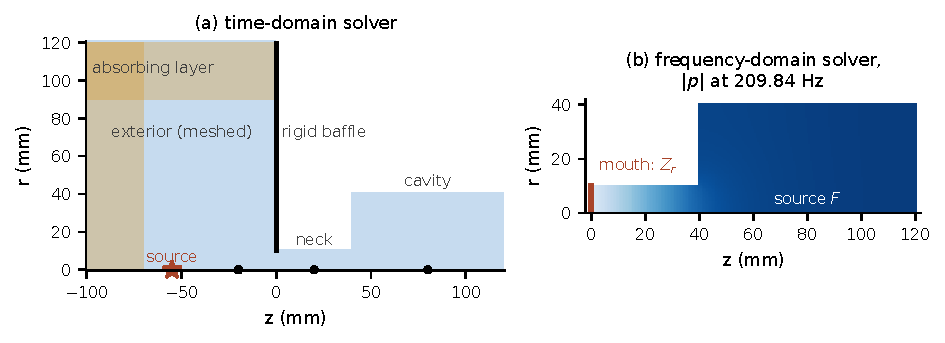
\includegraphics[width=\textwidth]{fig_domains.pdf}
  \caption{Computational domains on the meridian plane. (a) Time-domain solver: open neck,
  meshed exterior with a rigid baffle at $z=0$, absorbing layer (shaded) on the outer
  boundaries, Ricker source (star) and the three probes (dots). (b) Frequency-domain solver:
  the domain stops at the mouth, which carries the radiation impedance; colour shows $|p|$
  at 209.84~Hz on the 0.5~mm grid (\texttt{data/helmholtz\_mode.npz}).}
  \label{fig:domains}
\end{figure}

Both solvers use a uniform grid of step $h$ on the meridian plane (Fig.~\ref{fig:domains})
and the standard second-order stencil of the axisymmetric Laplacian, with the radial
part written as $4(p_1-p_0)/h^2$ on the axis.

\paragraph{Frequency domain} (\texttt{src/harmonic\_solver.py}). The operator of
Eq.~\eqref{eq:helmholtz} is assembled as a sparse complex matrix. A rigid wall is imposed by
folding the ghost node onto the diagonal: the coefficient of the missing neighbour is added
to the diagonal instead of appearing off-diagonal, which enforces a zero flux across the
face half a cell beyond the last fluid node. The Robin condition at the mouth eliminates the
ghost node through $p_{-1} = p_1 - 2h\alpha p_0$. Because $k^2$ and $\alpha$ depend on
$\omega$, each frequency requires a new sparse LU factorisation (SciPy \texttt{spsolve}):
0.1~s on the 1~mm grid (4\,961 nodes), 4~s on the 0.25~mm grid (77\,441 nodes). A Gaussian
volume source of width 10~mm drives the cavity; $f_0$ is the peak of the cavity pressure,
located by a three-point parabola on a 0.05~Hz sweep, and the radiation $Q$ is $f_0$ over the
$-3$~dB width. A second configuration of the same scheme, with the mouth set to $p=1$
(Dirichlet), is used in \texttt{notebooks/harmonic\_study.ipynb} for the neck-length study and
for Selamet's side-branch resonators, whose mouth is a pressure node at resonance.

\paragraph{Time domain} (\texttt{src/transient\_solver.py}). Equation~\eqref{eq:wave} is
advanced by explicit leapfrog with $\Delta t = 0.5\,h/(c\sqrt2)$. The Laplacian is written in
masked finite volumes: fluxes through faces between a fluid and a solid cell are zero, which
again places each wall on the face half a cell beyond the last node. The neck opens onto an
exterior of radius 120~mm and depth 100~mm terminated by 30~mm absorbing layers. A Ricker
pulse centred at 250~Hz is emitted 55~mm in front of the mouth, so the resonator is excited
over a broad band and rings at its own frequency after the pulse has passed. $f_0$ and $Q$
are obtained by fitting $A e^{-t/\theta}\cos(2\pi f_0 t+\phi)$ to the cavity probe for
$t \ge 45$~ms (\texttt{verification/grid\_convergence.py}), with $Q = \pi f_0 \theta$. The fit
locates $f_0$ well below the 4.9~Hz resolution of an FFT over the same window.

\paragraph{Outer boundaries} (\texttt{studies/radiation\_boundaries.py}). Three terminations
share one solver core: (i) a sponge, i.e.\ a damping term $\sigma\,\partial_t p$ with
$\sigma = \sigma_{\max} d^2$ across the layer, as in the original solver; (ii) the
first-order Mur condition $\partial_t p + c\,\partial_n p = 0$ on the outer ring
\citep{mur1981}; (iii) the unsplit PML \citep{grote2010}
\begin{equation}
\begin{aligned}
  \partial_t^2 p + (s_r+s_z)\,\partial_t p + s_r s_z\, p &= c^2\nabla^2 p + \nabla\cdot\boldsymbol{\psi},\\
  \partial_t \psi_r + s_r \psi_r = c^2 (s_z-s_r)\,\partial_r p, \qquad
  \partial_t \psi_z + s_z \psi_z &= c^2 (s_r-s_z)\,\partial_z p,
\end{aligned}
\end{equation}
with quadratic profiles $s_r$, $s_z$. This is the Cartesian stretch applied in the $(r,z)$
plane: the $1/r$ term of a cylindrical PML \citep{collino1998} is left out.

\paragraph{Neural-basis test} (\texttt{studies/neural\_basis\_benchmark.py}). For each family
of \basesHidden{} functions $\phi_j$ at random initialisation (tanh MLP, SIREN with
$\omega_0=5$ and 8, Gabor atoms, a three-zone partition of unity of sine networks in the
spirit of FBPINNs, and a Trefftz basis $J_0(\kappa_m r)Z_m(z)$), the frequency-domain field
$P$ at 209.84~Hz on the 1~mm grid is projected onto the span of $\{\phi_j\}$ by least
squares. Two numbers are reported: the relative field error of that projection, and the
residual $\lVert \nabla^2\tilde p + k^2 \tilde p + F\rVert / \lVert F\rVert$ of the
projection $\tilde p$ computed with automatic differentiation on 900 points of the fluid domain. A
residual of 100\% is what the zero field achieves. No network is trained in this test: it
measures the best that a basis allows, not what an optimiser finds.

% ===========================================================================
\section{Verification}
\label{sec:verification}

\subsection{Code verification: manufactured solutions}

\begin{figure}[t]
  \centering
  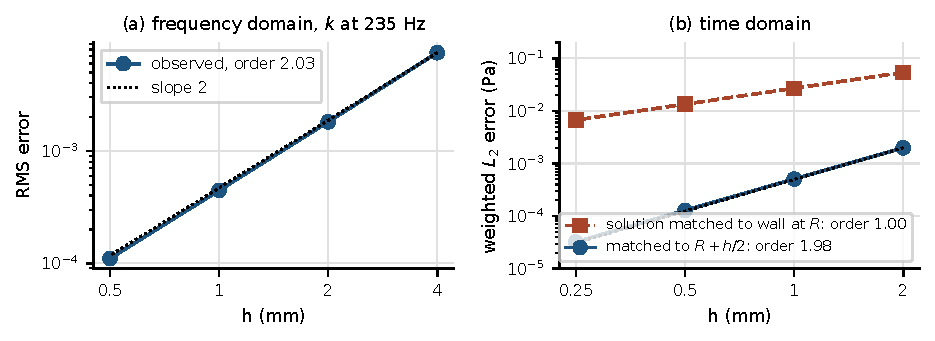
\includegraphics[width=\textwidth]{fig_mms.pdf}
  \caption{Manufactured solutions. (a) Frequency-domain scheme on a smooth domain with
  Dirichlet edges (\texttt{data/mms\_results.npz}). (b) Time-domain scheme with rigid walls
  (\texttt{data/mms\_transient.npz}): matched to the nominal wall position the error
  converges at first order; matched to the wall at $R+h/2$ it converges at second order.}
  \label{fig:mms}
\end{figure}

For the frequency-domain scheme, the solution $p_e=\cos(\pi r/R)\cos(\pi z/H)$ on a
$40\times120$~mm rectangle, regular on the axis, is imposed through its source term at the
wavenumber of 235~Hz. Over four grids from 4 to 0.5~mm the RMS error decreases at order
\mmsHarmonicOrder{} (Fig.~\ref{fig:mms}a). This test uses Dirichlet edges and therefore does
not exercise the wall treatment.

The time-domain test does. It uses $p = J_0(\lambda r)\cos\!\big(k_z(z+z_0)\big)\,T(t)$ in a
closed cylinder, with $\lambda$ chosen so that $\partial_r p=0$ on the lateral wall and $k_z$
so that $\partial_z p = 0$ on both ends, and $T(t)=u^3e^{-u}$, $u=t/\tau$, with $\tau$ matched
to the wave period so that $\partial_t^2 p$ and $c^2\nabla^2 p$ are of the same size.
When the manufactured solution places the walls at the nominal radius $R$ and height $H$,
the observed order is \mmsNominalOrder{} on four grids (Fig.~\ref{fig:mms}b). When it places
them at $R+h/2$ and $H+h$, the observed order is \mmsTransientOrder{} and the error at
$h=2$~mm is \mmsErrorRatio{} times smaller. The scheme is second order; the first-order error
comes from the wall position. The frequency-domain scheme has the same convention through
its ghost-node folding. Both solvers therefore simulate a resonator whose dimensions are
enlarged by $O(h)$, and raw frequencies at a single grid carry a bias of a few percent.

\subsection{Solution verification: grid convergence}
\label{sec:gci}

\begin{figure}[t]
  \centering
  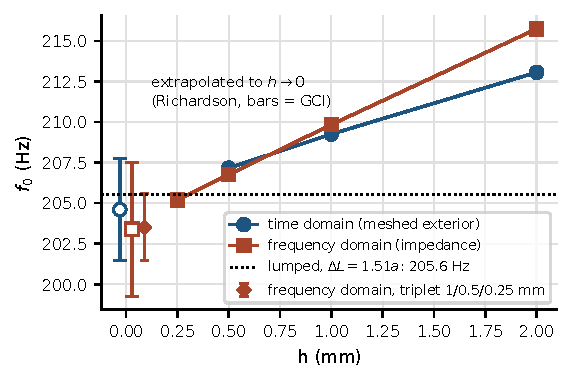
\includegraphics[width=0.66\textwidth]{fig_convergence.pdf}
  \caption{Natural frequency of the reference resonator against grid step for both solvers
  (\texttt{data/convergence\_f0.npz}, \texttt{data/fdm\_sweep\_h*.npz}), with the Richardson
  extrapolations at $h=0$ and their GCI, and the semi-empirical lumped reference.}
  \label{fig:convergence}
\end{figure}

On three grids with refinement ratio 2, the observed order $p$, the extrapolated value and
the fine-grid GCI are \citep{roache1994,celik2008}
\begin{equation}
  p = \frac{\ln\big|(f_3-f_2)/(f_2-f_1)\big|}{\ln 2},\quad
  f_{h\to0} = f_1 + \frac{f_1-f_2}{2^p-1},\quad
  \mathrm{GCI} = 1.25\,\frac{|f_2-f_1|/f_1}{2^p-1},
\end{equation}
with $f_1$ on the finest grid. Table~\ref{tab:gci} and Fig.~\ref{fig:convergence} give the
result on the reference geometry. Both solvers converge at an observed order close to 1,
as expected from the wall offset and from the staircase representation of the neck--cavity
junction. Extrapolated, they give \fExtPrec{} and \tExtPrec{}~Hz, \solverGapPrec\% apart,
which is inside both uncertainty bands. Their raw 1~mm values already agree to 0.3\%, but
both carry the same geometric bias, so that agreement alone says little; only the
extrapolated values are compared.

\begin{table}[t]
\centering
\caption{Grid convergence of $f_0$ (Hz) on the reference geometry. Time domain:
damped-sinusoid fit; frequency domain: peak of the response.}
\label{tab:gci}
\small
\begin{tabular}{lccccccc}
\toprule
solver & $h=2$ & $h=1$ & $h=0.5$ & $h=0.25$ mm & $p$ & $f_{h\to0}$ & GCI \\
\midrule
time domain (meshed exterior) & \tFA & \tFB & \tFC & -- & \tOrder & \tExtPrec & \tGCI\% \\
frequency domain (impedance) & \fFA & \fFB & \fFC & \fFD & \fOrder & \fExtPrec & \fGCI\% \\
\quad triplet 1 / 0.5 / 0.25 mm & & & & & \fOrderB & \fExtB & \fGCIB\% \\
\bottomrule
\end{tabular}
\end{table}

\paragraph{Fourth grid.} Three grids give exactly one observed order, so they cannot show
that the solution is in the asymptotic range. For the frequency-domain solver I added a
0.25~mm grid (\texttt{verification/control\_grid.py}). The second triplet gives $p=\fOrderB$
and moves the extrapolated value by \fExtShift\%, well inside the GCI. The same check was
done in the harmonic notebook with the Dirichlet mouth for $L=2$ and 4~cm: the observed
order goes from 0.91 to 1.00 and from 0.87 to 1.01, and the extrapolations move by 0.20\% and
0.36\%. A 0.25~mm time-domain run would take about 8~h on one core and was not done; the
time-domain extrapolation therefore rests on three grids.

\paragraph{Neck length.} With the Dirichlet mouth, the same three-grid study over five neck
lengths from 2 to 6~cm gives observed orders between 0.87 and 0.95 and GCIs between 2.0\%
and 2.3\% (mean 2.1\%; \texttt{notebooks/harmonic\_study.ipynb}, section 4). Fitted on those
extrapolated frequencies, a free power law $AL^b$ and the effective-length model
$A/\sqrt{L+\Delta L}$ cannot be told apart ($\Delta\mathrm{AICc}=0.3$); the effective-length
fit gives $\Delta L = 0.67a$, the interior correction used in the reference value.

\subsection{Outer boundary of the time-domain solver}
\label{sec:pml}

\begin{figure}[t]
  \centering
  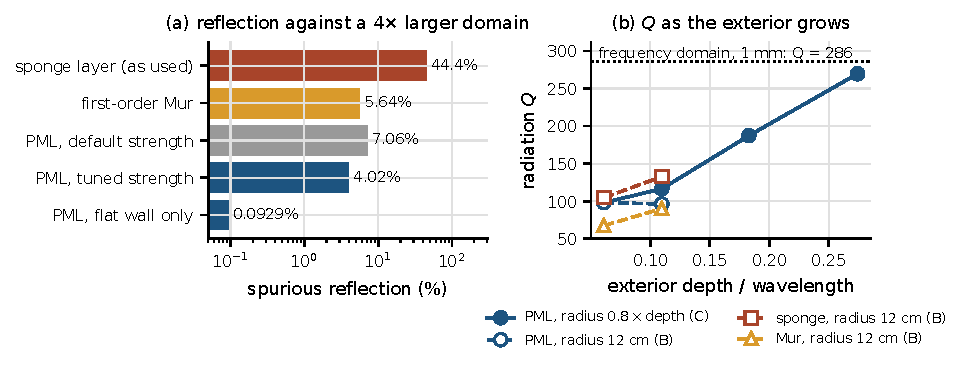
\includegraphics[width=\textwidth]{fig_boundaries.pdf}
  \caption{Outer boundaries (\texttt{data/pml\_study.npz}). (a) Spurious reflection of a
  4~kHz-centred Ricker pulse, measured at an off-axis probe against the same run on a domain
  four times larger. (b) Radiation $Q$ of the resonator as the exterior grows, against the
  $Q$ of the frequency-domain solver with the analytic impedance.}
  \label{fig:boundaries}
\end{figure}

The frequency was insensitive to the outer boundary, but the damping was not: with the
original sponge layer, the radiation $Q$ ranged from \spongeQmin{} to \spongeQmax{} as the
layer strength, thickness and domain size were changed on the 2~mm grid, while $f_0$ did not
move (\texttt{data/sponge\_sensitivity.npz}). To find out why, each termination was tested
on an empty exterior box: a pulse is fired towards the boundary and the probe signal is
compared with the same run on a domain four times larger, from which nothing can return
within the 1.4~ms window. The difference is the spurious reflection, with no analytic
reference needed.

\begin{table}[t]
\centering
\caption{Outer-boundary treatments. Reflection: peak spurious signal relative to the peak
incident signal. Drift: change in the radiation $Q$ of the resonator (1~mm grid) when the
exterior depth goes from 10 to 18~cm.}
\label{tab:pml}
\small
\begin{tabular}{lcc}
\toprule
treatment & spurious reflection & $Q$ drift, 10 $\to$ 18 cm \\
\midrule
sponge layer (original solver) & \reflSponge\% & $\driftSponge$\% \\
first-order Mur & \reflAbc\% & $\driftAbc$\% \\
PML (tuned strength) & \reflPml\% & $\driftPml$\% \\
\bottomrule
\end{tabular}
\end{table}

The sponge reflected \reflSponge\% of the incident amplitude (Table~\ref{tab:pml},
Fig.~\ref{fig:boundaries}a), enough to explain the spread in $Q$. The PML reflects
\reflPmlDefault\% at the default strength and \reflPml\% after scanning it, and its $Q$ moves
by $\driftPml$\% between the two exterior sizes, against $\driftSponge$\% for the sponge and
$\driftAbc$\% for the Mur condition. Running each wall alone isolates the limit of the PML:
\reflFlat\% ($\reflFlatdB$~dB) on the flat boundary $z=\mathrm{const}$, where the Cartesian
stretch is exact, and \reflCurved\% ($\reflCurveddB$~dB) on the cylindrical boundary, where
the $1/r$ term is missing. Neither a stronger profile nor a thicker layer lowers that floor.

A stable $Q$ between 10 and 18~cm is still not convergence. At 209~Hz the wavelength is
\wavelength~m, so the 10~cm exterior is \extFracA{} of a wavelength and the layer sits in the
reactive near field of the mouth. Growing the exterior to \extFracB, \extFracC{} and
\extFracD{} wavelengths takes $Q$ from \extQA{} to \extQB, \extQC{} and \extQD{}
(Fig.~\ref{fig:boundaries}b), approaching the $Q=\qImpedance$ of the frequency-domain solver
with the analytic impedance, while $f_0$ changes by \extFspread\%. The largest run is
consistent with convergence towards that value but does not demonstrate it.

% ===========================================================================
\section{Results}
\label{sec:results}

\subsection{The resonance and the end correction}

\begin{figure}[t]
  \centering
  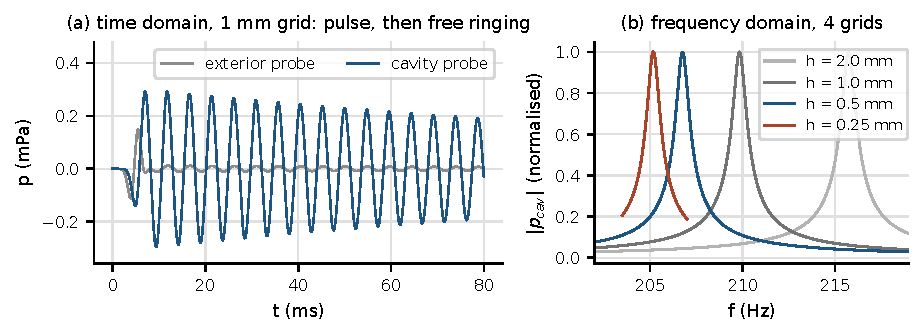
\includegraphics[width=\textwidth]{fig_resonance.pdf}
  \caption{(a) Time-domain solver, 1~mm grid: the pulse reaches the exterior probe, then the
  cavity keeps oscillating at its own frequency (\texttt{data/open\_resonator.npz}).
  (b) Frequency-domain response of the cavity on successive grids
  (\texttt{data/fdm\_sweep\_h*.npz}); the peak moves down as the walls move in.}
  \label{fig:resonance}
\end{figure}

In the time domain the resonator selects its frequency: after the pulse has passed, the
cavity rings at $f_0$ with no frequency imposed anywhere (Fig.~\ref{fig:resonance}a). In
the frequency domain the response is narrow: on the 1~mm grid the $-3$~dB width is \sweepBand~Hz. A first sweep at 1~Hz steps
read the peak at \sweepPeakCoarse~Hz and \sweepAmpCoarse~kPa; at 0.005~Hz steps it is
\sweepPeakFine~Hz and \sweepAmpFine~kPa, a 9\% error in amplitude because the step was wider
than the peak.

Inverting Eq.~\eqref{eq:lumped} gives the end correction implied by each frequency. From the
raw 1~mm time-domain value it is \dLraw$a$, 15\% below the $1.51a$ of the reference; from
the extrapolated value it is \dLext$a$, about 3\% above it. The apparent deficit of the
meshed exterior was the wall offset. With the impedance condition, the frequency-domain
study gives a shift in $\Delta L$ of $0.823a$ between the Dirichlet and the radiating mouth,
against $8a/(3\pi)=0.849a$ in Eq.~\eqref{eq:zr}. Since that reactance is imposed, this is a
consistency check of the chain, not an independent computation.

\subsection{Comparison with published measurements}
\label{sec:published}

\begin{figure}[t]
  \centering
  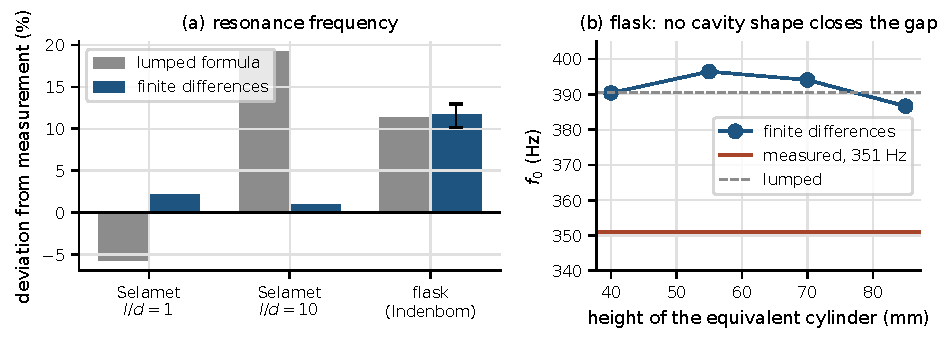
\includegraphics[width=\textwidth]{fig_validation.pdf}
  \caption{Comparison with published measurements (\texttt{data/literature\_validation.npz};
  Selamet values from \texttt{notebooks/harmonic\_study.ipynb}, section 5). (a) Deviation of
  the lumped formula and of the finite-difference solver; the bar on the flask spans the
  cavity aspect ratios tried. (b) Flask: finite-difference $f_0$ against the height of the
  equivalent cylindrical cavity.}
  \label{fig:validation}
\end{figure}

\begin{table}[t]
\centering
\caption{Resonance frequencies (Hz) against published measurements. Finite differences on
the 1~mm grid, no fitted parameter.}
\label{tab:published}
\small
\begin{tabular}{lcccc}
\toprule
case & measured & lumped, Eq.~\eqref{eq:lumped} & finite differences & deviation \\
\midrule
Selamet et al., $l/d=1$ & 91 & \selLumped & 93.0 & $+2.2\%$ \\
Selamet et al., $l/d=10$ & 72 & \selLumped & 72.7 & $+0.9\%$ \\
Indenbom \& Pogossian, flask & 351 & \flaskLumped & \flaskMin--\flaskMax & $+\flaskDevMin$ to $+\flaskDevMax\%$ \\
\bottomrule
\end{tabular}
\end{table}

Selamet et al.\ measured two concentric resonators with the same 4500~cm$^3$ cavity in two
shapes ($l/d=1$ and 10) and a neck of diameter 40.44~mm and length 85~mm \citep{selamet1997}.
They are side branches on a duct, so the neck sees a pressure node at resonance; they were
computed with the Dirichlet mouth. The lumped formula knows only the volume and returns
\selLumped~Hz for both, $\selLumpedDevA$\% and $\selLumpedDevB$\% from the measurements. The
two-dimensional field recovers both to 2.2\% and 0.9\% (Table~\ref{tab:published}). These
values are on the 1~mm grid, not extrapolated, and the deviations are of the size of the
GCI.

Indenbom and Pogossian measured an empty 100~mL Erlenmeyer flask at 351~Hz
\citep{indenbom2023}, where the lumped formula gives 391~Hz; my lumped model reproduces
\flaskLumped~Hz. The flask is conical and my cavity is a cylinder, so I replaced it by a
cylinder of equal volume and swept its aspect ratio. The solver stays between \flaskMin{}
and \flaskMax~Hz for every shape (Fig.~\ref{fig:validation}b), \flaskDevMin--\flaskDevMax\%
above the measurement. Resolving the field near the neck does not close the gap. In terms of
Eq.~\eqref{eq:lumped}, the measurement corresponds to an effective neck of about 54~mm
instead of 43~mm, which would be consistent with the neck flaring into the conical shoulder,
a geometry this solver cannot represent. I report this as an unexplained miss.

For damping, the same paper gives a half-width that brackets the measured $Q$ between
\qFlaskLo{} and \qFlaskHi{} (the paper does not state whether the width is taken at half
amplitude or half power). An estimate combining viscothermal losses in the neck and radiation
gives about \qFlaskPred{}: the model is optimistic, in the same direction as Moloney's
comparison \citep{moloney2004}. Neither solver contains viscothermal losses.

\subsection{Neural bases: a measured negative result}
\label{sec:bases}

\begin{figure}[t]
  \centering
  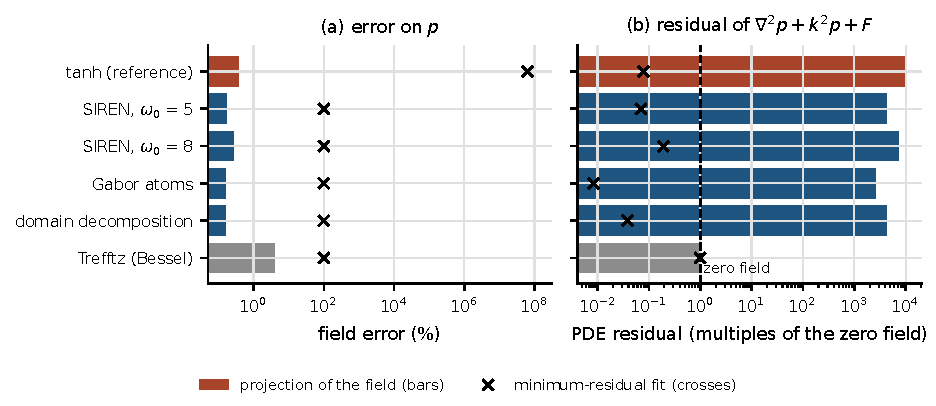
\includegraphics[width=\textwidth]{fig_bases.pdf}
  \caption{Least-squares projection of the verified field onto \basesHidden{} basis
  functions of each family (\texttt{data/bench\_bases.npz}). (a) Relative field error.
  (b) PDE residual of the same projection, normalised so that the zero field scores 100\%
  (dashed line).}
  \label{fig:bases}
\end{figure}

All neural bases represent the field well: the field error of the projection is between
\basesErrMin\% and \basesErrMax\% (Fig.~\ref{fig:bases}a). None represents its Laplacian: the
residual of the same projection is between \basesResMin{} and \basesResMax{} times that of the
zero field (Fig.~\ref{fig:bases}b). The conditioning of the residual operator varies by eleven
orders of magnitude between families (from $\kappaMin$ to $\kappaMax$), with sine
activations far better conditioned than tanh, yet the residual barely improves. The cause is
the structure of the solution: inside the cavity $\nabla^2 p$ and $-k^2 p$ are both large
and nearly cancel, so a 0.15\% error on $p$ becomes an error on $\nabla^2 p$ larger than the
source itself. The Trefftz basis is the counter-example: each function satisfies
$\nabla^2\phi + k^2\phi = 0$ exactly, so its residual equals that of the zero field
(\trefftzRes\%), but it cannot represent the source and fits the field only to
\trefftzErr\%.

% ===========================================================================
\section{Discussion and limitations}

\paragraph{What the results support.} Two solvers with different discretisations and
different radiation models agree on the natural frequency of the reference resonator to
\solverGap\%, inside their grid uncertainties of about 2\%, and the frequency-domain scheme
reproduces two published resonators to within that uncertainty. The verification sequence
found an error that the cross-check alone would have hidden: both solvers carry the same
half-cell wall offset, so their raw values agree better than either agrees with its own
converged value.

\paragraph{What they do not support.}
\begin{itemize}
  \item \emph{Damping.} Both solvers are lossless. The viscothermal boundary layer in the
    neck (about 0.14~mm at this frequency) is the dominant loss and is only estimated
    analytically. The $Q$ values above are radiation-only and are not predictions of a real
    resonator.
  \item \emph{Grid convergence.} Observed orders near 1 come from the wall offset and the
    staircase walls, so the GCI is a first-order estimate. The time-domain extrapolation
    rests on three grids.
  \item \emph{Geometry.} Cavities are cylinders. The flask miss is consistent with its
    conical shoulder, but this has not been shown.
  \item \emph{Outer boundary.} The Cartesian PML has a 4\% reflection floor on the curved
    boundary, and the reflection was measured with a 4~kHz-centred pulse, whose wavelength
    is much shorter than at the resonance. The radiation $Q$ of the time-domain solver is
    not converged in exterior size.
  \item \emph{Comparison data.} All measurements are other authors'. Two of the three cases
    are side-branch resonators computed with a Dirichlet mouth on a single grid.
  \item \emph{Neural bases.} The test measures projections onto fixed random bases, not
    trained networks, and the target is the 1~mm finite-difference field, which itself
    satisfies the continuous equation only to discretisation accuracy.
\end{itemize}

% ===========================================================================
\section{Conclusion and future work}

A finite-difference model of an open Helmholtz resonator predicts its natural frequency
with a stated uncertainty of about 2\%, provided that the half-cell wall offset revealed by
the manufactured solution is extrapolated away. The end correction computed by the meshed
exterior, \dLext$a$, is within about 3\% of the semi-empirical value, and two published
resonators are reproduced to 0.9--2.2\%. One published resonator is missed by about 11\%,
and damping is outside the scope of these lossless models. The next steps are a cylindrical
PML to remove the 4\% floor, a body-fitted or cut-cell wall treatment to recover second-order
convergence, a viscothermal boundary-layer model in the neck, and a ring-down measurement of
a real resonator, for which the protocol and analysis script are in the repository.

% ===========================================================================
\section*{Reproducibility statement}

All code, data and figures are in the repository. The figures and the numbers quoted in the
text are produced by \texttt{python paper/make\_figures.py} from versioned files in
\texttt{data/}, and the report is built by \texttt{paper/build\_paper.sh}. Main commands and
times on the machine used (Intel Core i7-6700HQ, 4 cores, 32~GB RAM, Windows~10; Python
3.11.9, NumPy 2.2.6, SciPy 1.15.2, Matplotlib 3.10.6, PyTorch 2.8.0 CPU; one core per run):
\begin{itemize}\itemsep0pt
  \item \texttt{verification/mms\_transient.py}: transient MMS, 15~s.
  \item \texttt{src/transient\_solver.py} with \texttt{OR\_TMS=250} and \texttt{OR\_H} set to
    2, 1 and 0.5: the three time-domain runs, about 1, 5 and 40~min (scaled from timed short
    runs); then \texttt{verification/grid\_convergence.py}.
  \item \texttt{studies/frequency\_sweep.py} with \texttt{SW\_DF=0.05}: over 195--220~Hz with
    \texttt{SW\_H} set to 2, 1 and 0.5 (under 1, 1 and 6~min), and over 203.5--207~Hz with
    \texttt{SW\_H=0.25} (71 solves, 9~min on a loaded machine); then
    \texttt{verification/control\_grid.py}.
  \item \texttt{studies/radiation\_boundaries.py}: part A (reflection) a few minutes, parts
    B and C several hours.
  \item \texttt{experiments/literature\_validation.py}: about 4~min.
  \item \texttt{studies/neural\_basis\_benchmark.py}: under 1~min.
  \item \texttt{notebooks/harmonic\_study.ipynb}: Dirichlet-mouth study, MMS, Selamet cases.
\end{itemize}

\bibliographystyle{abbrvnat}
\bibliography{references}

\end{document}
